\documentclass[letterpaper,10pt]{article}
\usepackage{graphicx}

\title{Angular contact with TensorFlow}
\author{Rocco Malisi}

\begin{document}
	\maketitle
	\newpage
	
	\begin{abstract}
		Abstract text alsdjfsdalsdjlfksdjlk
	\end{abstract}
	\newpage
	
	\tableofcontents
	\newpage
	
	\section{Introduction}
	\section{Methods}
	\section{Results}
	\subsection{Performing an EDA on the first angular contact dataset}
	To get a better understanding of dataset \#1, an EDA is performed. The objective is to identify patterns and relationships in the data. The insights gained by this analysis will be used in building and improving the model.\newline
	The dataset consists of three columns and 1365 rows. The columns are 'Fr' (radial force in N[Newton]), 'n' (rotational speed in rpm[revolutions per minute]) and 'Lifetime' (lifetime	in h[hours]) \newline
	In the first step, the univariate properties of the variables are explored.
	Figure 1 shows a plot of Fr. Fr starts at 200 and is increased by 100 every 35 rows throughout the whole dataset. The final and highest value of Fr is 4000.
	
	     
	
	\begin{figure}
		\caption{Plot of Fr}
		\centering
		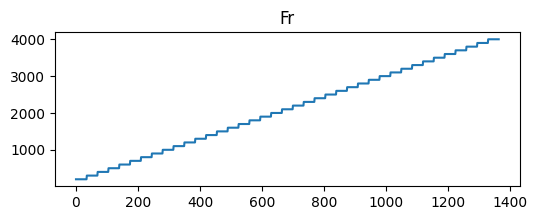
\includegraphics[scale=0.65]{assets/dataset1_column_Fr_plot.png}
	\end{figure}
	\begin{figure}
		\caption{Plot of Lifetime}
		\centering
		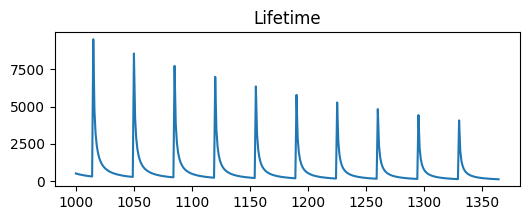
\includegraphics[scale=0.65]{assets/dataset1_column_Lifetime_plot2.png}
	\end{figure}
	\begin{figure}
		\caption{Plot of Lifetime}
		\centering
		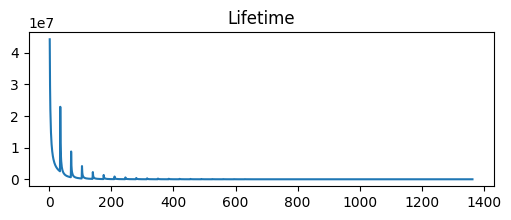
\includegraphics[scale=0.65]{assets/dataset1_column_Lifetime_plot1.png}
	\end{figure}
	\begin{figure}
		\caption{Plot of n}
		\centering
		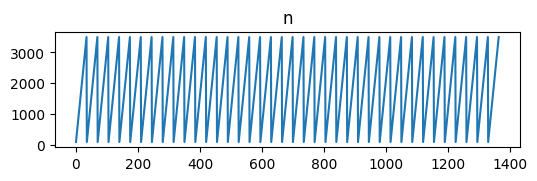
\includegraphics[scale=0.65]{assets/dataset1_column_n_plot.png}
	\end{figure}

	
	\newpage
	\bibliographystyle{plain} 
	\bibliography{bibliography}
	
\end{document}